\documentclass[11pt]{article}
\usepackage[document]{ragged2e}
\usepackage[letterpaper, margin = 1in]{geometry}
\usepackage[utf8]{inputenc}
\usepackage{parskip}
\usepackage{circuitikz}
\usepackage{mathtools}
\usepackage{graphicx}
\usepackage{amsmath}
\usepackage{physics}
\usepackage{epstopdf}
\usepackage{indentfirst}
\usepackage{multicol}
\setlength{\columnsep}{1cm}
\usepackage{wrapfig}
\usepackage{subcaption}
\usepackage{fancyhdr}
\usepackage{siunitx}

\pagestyle{fancy}
\fancyhf{}
\rhead{pydls}
\lhead{\textbf{Thy Doan Mai Le}}
\cfoot{\thepage}
%%%%%%%%%%%%%%%%%%%%%%%%%%%%%%%%%%%%%
%	TITLE
\begin{document}
\begin{titlepage}
    \begin{center}
        \vspace*{0.5cm}
      	\LARGE{\textbf{Department of Physics $\&$ Astronomy}}\\
      	\vspace{0.2cm}
      	\textbf{Ithaca College}\\
      	
      	\vspace{5cm}
      	\textbf{\LARGE{pydls }}\\
	\vspace{0.5cm}
      	\textbf{\LARGE{A Python Suite for the Bayesian Inferrence of Particle Size Distributions in Dynamic Light Scattering Experiments}}\\
      	\vspace{4cm}
	
      	\normalsize{
      	 Thy Doan Mai Le\\
	 Advisor: Jerome Fung\\
	 \vspace{4cm}
      	Date: \today\\}
      	\vspace{2cm}
      	
      
    \end{center}
\end{titlepage}
%%%%%%%%%%%%%%%%%%%%%%%%%%%%%%%%%%%%%
\tableofcontents

\newpage
% INTRODUCTION
\section{Dynamic Light Scattering}
\justifying
\indent Dynamic ligh scattering (DLS) is a technique used to determine the size distribution of a sample of particles suspended in an optically transparent medium, also known as a colloidal sample. When incident light is directed towards a colloidal sample, each particle within the sample scatters the incident light independently and this same process repeats for all of the particles within the sample. A sample schematic of a DLS experiment is found in Fig.~\ref{fig:dls-general-setup}. Because each molecule experiences random Brownian motion while suspended in the sample, the intensity of the scattered light fluctuates as these molecules move about. A similar phenomenon occurs with starligh in the night sky. When ligh from distant stars reaches the Earth's atmosphere, the particles in the atmostphere scatter this light. These particles are not stationary, however, but move about constantly in a randomized fashion. As a result, the scattered starlight is sometimes brighter, sometimes dimmer and our eyes register this fluctuation as ``twinkling" stars. 

\begin{figure}
\centering
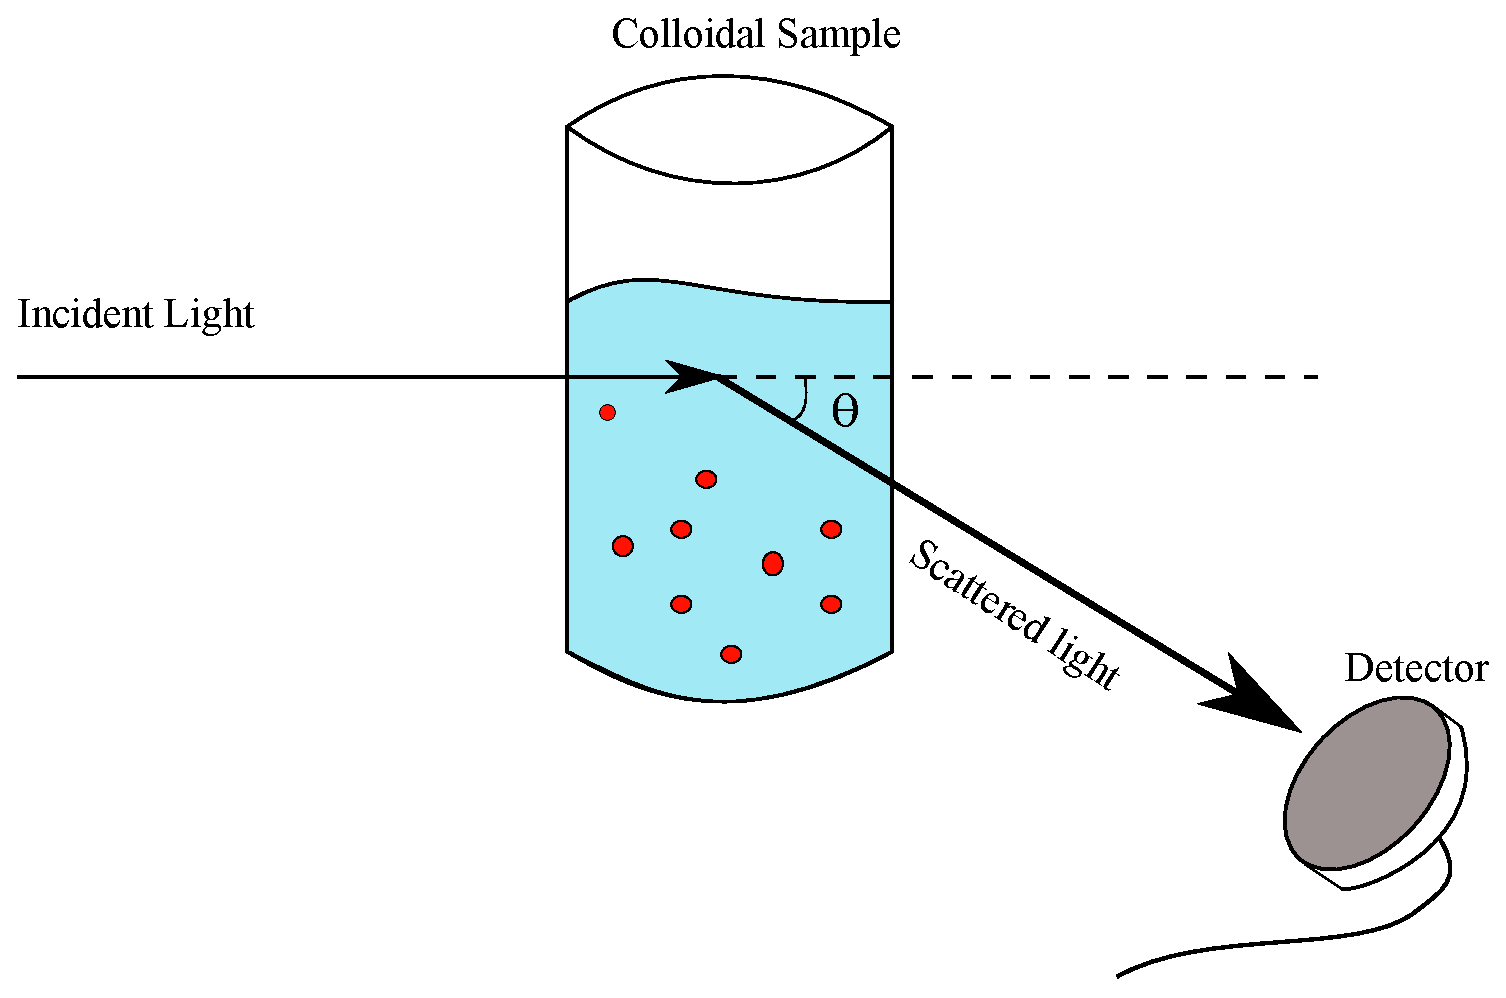
\includegraphics[width=0.8\linewidth]{dls-general-setup.eps}
\caption{When incident light encounters the colloidal sample, it is scattered by each individual particulate molecule within the sample and upon exiting the sample, all individually scattered light rays come together to give an interference pattern that is then received by the detector. Because the individual particles within the sample all experience random Brownian motion, the interference pattern is predicted to have a fluctuating intensity as the molecules move into and out of the incident light beam.}
\label{fig:dls-general-setup}
\end{figure}


For colloidal samples, the scattered light also ``twinkles" and the ``twinkling" pattern is actually distinct depending on the size, shape and other physical properties of the particles in the sample. Larger particles experience more drag during Brownian motion due to their larger surface area. Due to the larger drag, their Brownian motion occurs in a more gradual fashion over time. Because these larger particles are moving much more slowly, they produce scattered light that ``twinkles", or fluctuates in intensity, very gradually over time. Smaller particles, because they experience a much smaller drag due to their reduced size, move about very quickly, changing their position very rapidly in time. As a result, the scattered light from smaller particles fluctuates in intensity very quickly. 

\begin{figure}
\centering
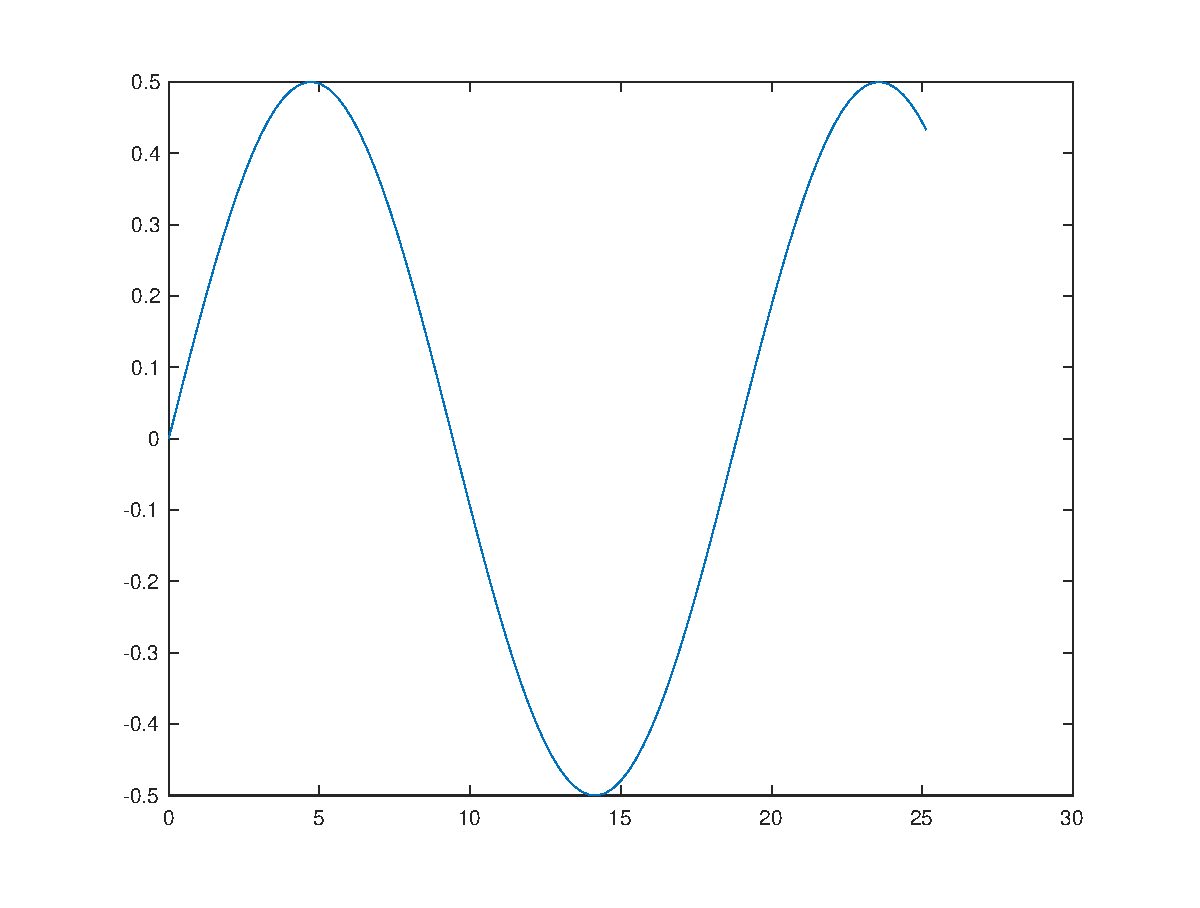
\includegraphics[width=0.4\linewidth]{large-particle-intensity.eps}
\caption{Large particles experience more drag and change their positions much more slowly than smaller particles. As a result, the scattered light's intensity changes very slowly with time. If the particle was moving in a sinusoidal motion, then the scattered light's intensity would have a similar, slowly varying sinusoidal pattern.}
\label{fig:large-particle-intensity}
\end{figure}

\begin{figure}
\centering
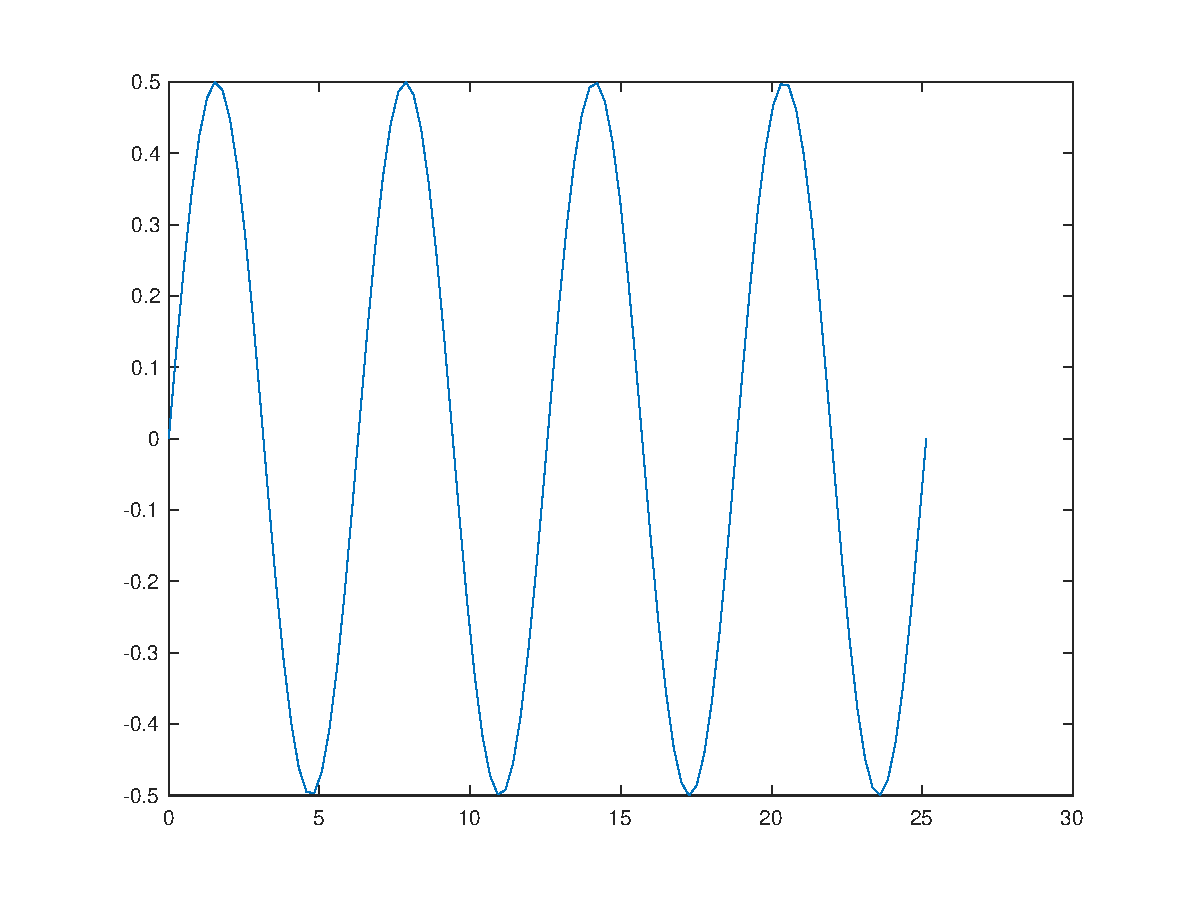
\includegraphics[width=0.4\linewidth]{small-particle-intensity.eps}
\caption{Smaller particles experience less drag and thus change their positions much faster than larger particles. Because of that, the light that they scatter has a very rapidly changing intensity. If the small particle was moving in a sinusoidal motion with a very high frequency (which is typical of a fast moving particle), the scattered light intensity will have a sinusoidal pattern with a high frequency as well.}
\label{fig:small-particle-intensity}
\end{figure}

In real-world situations, particles in Browninan motion do not have perfectly sinusoidal and periodic trajectories that scatter light so that the resultant intensity is perfectly periodic. Typically, scattered light from colloidal samples often have an aperiodic pattern with a lot of noise added in. In order to extract any useful information from the fluctuating scattered light, the scattered light's intensity that is detected by the detector in Fig.~\ref{fig:dls-general-setup} is used to produce an autocorrelation function. A correlation function demonstrates the degree of similarity between two consecutive data points in a data set. In the case of DLS experiments, the correlation function is expected to be an exponential decrease because over time, fluctuations in the detected signal cause the similarity between consecutive data points to dramatically fall. As a result, the correlation function takes a nosedive and resembles an exponential drop. In order to extract useful information about the colloidal sample, mathematical models are fit against the correlation function. In this project, the mathematical model proposed by Buoalem, Jabloun, Ravier, Naiim and Jalocha is used in an implementation of Monte Carlo Markov chain to infer the particle size distribution of a colloidal sample, given its autocorrelation function from a DLS experiment at one single angle. 

%%%%
\section{Theoretical Background}
\subsection{Prior Distribution}
According to Buoalem, Jabloun, Ravier, Naiim and Jalocha, the prior distribution of this non-parametrized method is as follows:

\begin{equation}\label{eq:prior}
p(\mathbf{f}) \propto exp\left( \mathbf{f}^{T} \mathbf{L_2}^{T}\mathbf{L_2}\mathbf{f} \right), \textrm{if } \mathbf{g} \geq 0
\end{equation}

\subsection{Likelihood Distribution}
The likelihood distribution is modeled according to the $g^{(2)}$ function as 

\begin{equation} \label{eq:likelihood}
p(\mathbf{\tilde{g}^{(2)}} | \mathbf{f}, \sigma^{2}_r ) = \frac{1}{{(2\pi)}^{\frac{M_r}{2}} \sigma^{M_r}}exp\left( -\frac{\chi_r(\mathbf{f})}{2\sigma^2_r}\right)
\end{equation}
if $\mathbf{f} \geq 0$.

The $\chi$-squared $\chi_r(\mathbf{f})$ is defined as 

\begin{equation}
\chi_r(\mathbf{f}) = \sum_{j=1}^{M_r} {\left( \tilde{g}_{\theta_r}^{(2)} (\tau_j) - g_{\theta_r}^{(2)} (\tau_j) \right)}^2
\end{equation}

\subsection{Posterior Distribution}
With the prior and likelihood distributions described in Eq.~\ref{eq:prior} and Eq.~\ref{eq:likelihood}, the posterior distribution for the particle size distribution with the noise variance given the measured autocorrelation data ($g^{(2)}$) is: 

\begin{equation}\label{eq:posterior}
p(\mathbf{f}, \sigma_1^2,\ldots, \sigma_r^2|\mathbf{\tilde{g}^{(2)}}) \propto exp \left( -\mathbf{f}^T\mathbf{L_2}^T\mathbf{L_2} \right) \prod_{r=1}^{R} \left[ \frac{1}{\sigma_r^{M_r+2}} exp \left( -\frac{\chi_r(\mathbf{f})}{2\sigma_r^2} \right) \right]
\end{equation}

Using the classical Jeffrey prior density for the noise variance in $\mathbf{\tilde{g}^{(2)}}$,
\begin{equation}\label{eq:noisevariance}
p(\sigma_r^2) \propto \frac{1}{\sigma_r^2}
\end{equation}
the posterior distribution can be integrated over the noise variance with the following integral:

\begin{equation} \label{eq:originalIntegral}
\int_{0}^{\infty} \frac{1}{\sigma_r^{M_r + 2}} exp \left( -\frac{\chi_r(\mathbf{f})}{2\sigma_r^2} \right)d\sigma_r
\end{equation}
 
 In order to integrate this integral, let $\sigma_r = \frac{1}{t}$ and thus $d\sigma_r = -\frac{1}{t^2}dt$. From this, we can rewrite expressions from the integrand in Eq.~\ref{eq:originalIntegral} as follows.
  \begin{equation}
 \begin{split}
 \frac{1}{\sigma_R^{M_r + 2} } & = t^{M_r + 2} \\
 \frac{\chi_r(\mathbf{f})}{2\sigma_r^2} & = \frac{\chi_r(\mathbf{f})}{2} t^2
 \end{split}
 \end{equation}
 Thus the integral from Eq.~\ref{eq:originalIntegral} becomes:
 \begin{equation} \label{eq:substitution1}
 \begin{split}
&  \int_{\infty}^{0} t^{M_r + 2} \left( -\frac{1}{t^2} \right)exp \left( -\frac{\chi_r(\mathbf{f})}{2} t^2 \right) dt \\
& =  \int_{0}^{\infty} t^{M_r}exp\left( -\frac{\chi_r(\mathbf{f})}{2} t^2 \right) dt
 \end{split}
 \end{equation}
 The limits switched from (0, $\infty$) in Eq.~\ref{eq:originalIntegral} to ($\infty$, 0) in Eq.~\ref{eq:substitution1} because of the substitution $\sigma_r = \frac{1}{t}$. The reciprocal relationship of the substitution switched the limits of the integration. In order to make the integral easier to integrate, the minus sign on the second line of Eq.~\ref{eq:substitution1} is exchanged for the re-switching of the integration limits from ($\infty$, 0) back to (0, $\infty$). 
 
 In order to actually integrate Eq.~\ref{eq:substitution1}, a second substitution has to be made. Let $\tau = t\sqrt{\chi_r}$ and d$\tau = \sqrt{\tau}$dt. From this, we can rewrite the expressions in the integrand of Eq.~\ref{eq:substitution1} as follows. 
 \begin{equation}
 \begin{split}
 \chi_r(\mathbf{f}) t^2 & = \tau^2 \\
 t^{M_r} & = {\left( \frac{\tau}{\sqrt{\chi_r}} \right)}^M_r \\
 & = \tau^{M_r}\chi_r^{-\frac{M_r}{2}} 
 \end{split}
 \end{equation}
 
 From the above substitutions, the integral becomes:
\begin{equation}
\begin{split}
 & \int_{0}^{\infty}\chi_r^{-\frac{1}{2}} \tau^{M_r} \chi_r^{-\frac{M_r}{2}} exp\left( -\frac{\tau^2}{2} \right) d\tau \\
& = \int_{0}^{\infty} \chi_r^{-\frac{1}{2}(M_r + 1)} \tau^{M_r} exp\left( -\frac{\tau^2}{2} \right) d\tau
\end{split}
\end{equation}

Since the $\chi_r$ term does not have $\tau$ dependence, we can pull that out of the integrand, giving us the following integral at the end:
\begin{equation}
\chi_r^{-\frac{1}{2}(M_r + 1) }\int_{0}^{\infty}\tau^{M_r}exp\left( -\frac{\tau^2}{2} \right) d\tau
\end{equation}

Recall that the $\chi_r$ expression was previously 
\begin{equation}
\chi_r(\mathbf{f}) = \sum_{j=1}^{M_r} {\left( \tilde{g}^{(2)}_{\theta_r} (\tau_j) - g^{(2)}_{\theta_r}(\tau_j) \right)}^2
\end{equation}
where $\tilde{g}^{(2)}$ is modeled to be:
\begin{equation} \label{eq:g2}
\begin{split}
 \tilde{g}^{(2)}_{\theta_r} (\tau_j) & = 1 + \beta_r {\left( k_{\theta_r}\sum_{i=1}^{N}f(D_i) C_{I,\theta_r}(D_i) exp\left( -\frac{\Gamma_{0,\theta_r}}{D} \tau_j \right) \Delta D_i \right)}^2 \\
\text{where } \Gamma_{0,\theta_r} & = \frac{16\pi n^2 \sin^2(\theta/2)k_B T}{2\lambda_0^2\eta}
 \end{split}
\end{equation}

with 

\begin{equation}
\begin{split}
& \text{n } : \text{refractive index}\\
& \theta\text{ : angle at which scattered light was measured}\\
& k_B\text{ : Boltzmann constant} \\
& T\text{ : temperature in Kelvin} \\
& \lambda_0\text{ : incident wavelength value in vacuum}\\
& \eta\text{ : viscosity} \\
& D_i\text{ : diameter of particle size}\\
& \beta_r\text{ : instrumental factor}\\
& k_{\theta_r}\text{ : normalization constant that can be found via k = }\frac{1}{\int_{0}^{\infty} f(D)C_{I,\theta}(D) dD}\\
&\tau_j\text{ : delay times} \\
&f(D)\text{ : the particle size distribution function}
\end{split}
\end{equation}

The posterior distribution is now defined to be:
\begin{equation}
p(\mathbf{f}|\tilde{\mathbf{g}}^{(2)}) \propto exp\left( -\mathbf{f}^T\mathbf{L_2}^T \mathbf{L_2}\mathbf{f}\right) \prod_{r=1}^{R} {\left[\chi_r(\mathbf{f})\right]}^{-\frac{M_r}{2}}
\end{equation}

Since $\chi_r(\mathbf{f}) = \sum {\left( \tilde{g}^{(2)}_{\theta_r} (\tau_j) - g^{(2)}_{\theta_r}(\tau_j) \right)}^2$, the posterior distribution is essentially:
\begin{equation}
p(\mathbf{f}|\tilde{\mathbf{g}}^{(2)}) \propto exp\left( -\mathbf{f}^T\mathbf{L_2}^T \mathbf{L_2}\mathbf{f}\right) \prod_{r=1}^{R} {\left( \sum{(\tilde{g}^{(2)}_{\theta_r} (\tau_j) - g^{(2)}_{\theta_r}(\tau_j) )}^2 \right)}^{-\frac{M_r}{2}}
\end{equation}

When the log of the posterior is taken, the above equation becomes:
\begin{equation}
\ln(p) = -\mathbf{f}^T\mathbf{L_2}^T \mathbf{L_2}\mathbf{f} + \left(-\frac{M_r}{2} \right) \ln \left(\sum {\left( \tilde{g}^{(2)}_{\theta_r} (\tau_j) - g^{(2)}_{\theta_r} (\tau_j) \right)}^2 \right)
\end{equation}


%%%%%%%%%%%%	
	
\section{Development}

In order to test the functionality of pydls, the package was used to infer simulated monodisperse and bidisperse Gaussian particle size distributions. Each simulated particle size distribution (PSD) is first used to generate a $g^2$ function as described in Eq.~\ref{eq:g2}, which is then is fitted using the exponential decay model to estimate the approximate mean and formulate a Gaussian distribution around this mean, as if we had no idea what the original PSD looked like. The $g^2$ data is now fed into the infer function in the pydls package with the approximated PSD as starting point for the MCMC walkers. The infer function will then give results from all of its walkers and utility functions within pydls can be used to extract the final particle size distribution, which will then be compared to the original, simulated PSD. 

\subsection{Bidisperse Distribution}
The following self-generated particle size distribution with two peaks of different full-width-half-max (FWHM) values was used to test the validity of the $g^{(2)}$ function on a bimodal distribution. The reason for this test is to verify that the implementation written is able to work with a bimodal size distribution, since one of the advantages of the Direct Bayesian Method (DBM) is that it is able to work with almost any particle size distribution. 

\begin{figure}
\centering
\includegraphics[width=0.5\linewidth]{bidisperse_psd.png}
\caption{The distribution of particle size (not normalized here) has a peak at $3.33\times10^{-7}$\si{meter} and another peak at $6.66\times10^{-7}$\si{meter}}
\label{fig:bidisperse_psd}
\end{figure}

From this distribution, the $g^{(2)}$ autocorrelation function of intensity v. time was found to be:

\begin{figure}
\centering
\includegraphics[width=0.5\linewidth]{g2.png}
\caption{The $g^{(2)}$ autocorrelation function extrapolated from the implementation.}
\label{fig:g2_model}
\end{figure}

In order to verify the validity of this autocorrelation function, I used SciPy's optimization for curve fits to extrapolate, from this autocorrelation function, the single exponential decay and the method of cummulants models. The goal of this method of testing is to verify that both of the single exponential decay and cummulants models fail upon the emergence of a bimodal particle size distribution. In order to detect this anticipated failure, the residuals between the $g^{(2)}$ model and each of the tested models (single exponential/cummulants) are plotted. Failure of each of the tested models is present when overshooting and/or undershooting are present in the residuals plot. 

When tested against the single exponential decay model, the residuals plot is depicted in Fig.~\ref{fig:expo_residuals}.

\begin{figure}
\centering
\includegraphics[width=0.5\linewidth]{expo_residuals.png}
\caption{The undershooting and overshooting are both apparent around the region of exponential decay, implying that the exponential fit is unable to capture certain aspects of the autocorrelation. This is congruent with the given data. Since single exponentials are only able to capture information of systems with 1 single particle size, a bimodal distribution of particle size should render the single exponential model inept.}
\label{fig:expo_residuals}
\end{figure}

When tested against the cummulants model, the residuals plot is as depicted in Fig.~\ref{fig:cummulants_residuals}.

\begin{figure}
\centering
\includegraphics[width=0.5\linewidth]{cummulants_fit_residuals.png}
\caption{The residuals between the autocorrelation and the cummulants fit model showed dramatic breakdown around the exponential decay region, signifying that the cummulants fit was not able to truly capture the $g^{(2)}$ information.}
\label{fig:cummulants_residuals}
\end{figure}

In conclusion, the residuals plots have shown that both the single exponential and the cummulants model were unable to fully capture the information displayed in the $g^{(2)}$ autocorrelation and therefore should not be used in analyzing dynamic light scattering information of samples with know multimodal particle size distributions. 

\subsection{Single Gaussian distribution}
Write about tests of the g(2) model using a single Gaussian distribution of particle sizes. In this test, the expected results are that the method of cumulants and the single exponential model both fail to completely capture the physics, shown by a residual plot that exhibits overshooting and undershooting of results.

%%%%%%%%%%%%%%%%%%%%%%%%%%%%%%%%%%%%%%%%%%%%%%%%%%%%

%%%%%%%%%%%%%%%%%%%%%%%%%%%%%%%%%%%%%%%%%%%%%%%%%%%%%%%%
% Actual Testing 
% with 2015_07_22_Eonly0005 asc data
%%%%%%%%%%%%%%%%%%%%%%%%%%%%%%%%%%%%%%%%%%%%%%%%%%%%%%%%

\subsection{Bayes Take 20 - July 8, 2019}
\begin{figure}
\centering
\includegraphics[width=0.4\linewidth]{take20.png}
\caption{The simulated particle size distribution with a mean of $4.488\times10^{-9}$ and a standard deviation of $6.67\times10^{-11}$.}
\label{fig:take20simulated}
\end{figure}

After 19 previous rounds of debugging, the package was finally stable and ready for testing using a variety of particle size distributions: narrow, wide, monodisperse or bidisperse. In Bayes Take 20, performed on July 08, 2019, the simulated particle size distribution has a mean at $4.488\times10^{-9}$ and a standard deviation of $6.67\times10^{-11}$. Throughout all following tests, environmental conditions are kept to be:

\begin{itemize}
	\item m = 20
	\item c = 1
	\item $\eta$ = $1\times10^{-3}$
	\item $\theta$ = $\pi$/2
	\item n = 1.33
	\item $k_B$ = $1.38\times10^{-23}$
	\item T = 298.15\si{\kelvin}
	\item $\lambda_0$ = $638\times10^{-9}$
	\item $\beta$ = 1
\end{itemize}

Using the g2 data as well as the simulated PSD, the inference was able to successfully yield a PSD, as depicted in Fig.~\ref{fig:take20infer}, that resembled the original simulated PSD, albeit with some sharp, small magnitude peaks in locations that previously had zero probability in the original PSD. 

\begin{figure}
\centering
\includegraphics[width=0.4\linewidth]{take20infer.png}
\caption{The inferred particle size distribution using pydls on the g2 data in Fig.~\ref{fig:take20g2} and the environmental factors above.}
\label{fig:take20infer}
\end{figure}


\begin{figure}
\centering
\includegraphics[width=0.4\linewidth]{take20g2.png}
\caption{The g2 function using the stimulated particle distribution and the environmental factors as described above.}
\label{fig:take20g2}
\end{figure}

\subsection{Further Testing}
Further testing can be found at \verb#https://github.com/thydmle/pydls/tree/master/Test#, starting with Bayes Take 21 and finishing at Bayes Take 33. 

\section{Conclusion}
Comprehensive testing showed that pydls is successfully able to handle DLS autocorrelation functions from single angle data with very high accuracy. Further development should target the expansion of this package into a code base that is able to handle multi-angle DLS data with accurate (instead of an approximation) Mie scattering coefficient calculations.

\end{document}